
\chapter{Single-core Design}
\label{sec:singlecore}
\startcontents[chapters]
\printcontents[chapters]{}{1}{}

\section{Introduction}
While the majority of this report will focus on the multi-processing functionality of this project, it is important understand the design decisions of the single core to understand the features and limitations of the multi-core system-on-chip as a whole.

\section{Design and Implementation}
The single-core design is a traditional 5-stage RISC processor (fetch, decode, execute, memory, write-back). The core uses separate instruction and data memories in the style of a Harvard architecture \cite{harvard}.

To satisfy \ref{cd:vendor}, the Verilog code will be self-contained in a single file. This reduces the hierarchical complexity and eases cross-vendor project set-up as only a single file is required to be included. 

\begin{figure}[H]
\centering 
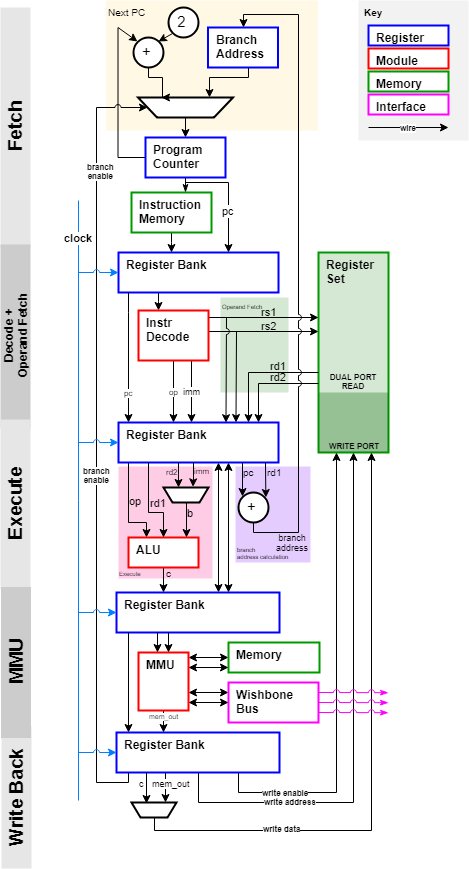
\includegraphics[width=10cm]{../img/risc}
\caption{Vmicro16 RISC 5-stage RTL diagram showing: instruction pipelining (data passed forward through clocked register banks at each stage); branch address calculation; ALU operand calculation (rd2 or imm); and program counter incrementing.}
\label{fig:risc}
\end{figure}

A small reduction in size within the single-core will result in substantial size reductions in 

\subsection{Instruction Set Architecture}
\begin{quotation}
\noindent Core deliverable \ref{cd:isa} details the background for the requirement of a custom instruction set architecture. 
The 16-bit instruction set listing is shown in \cref{fig:isa}.
\end{quotation}

In this proposed architecture, most instructions are \textit{destructive}, meaning that source operands also act as the destination, hence effectively \textit{destroying} the original source operand. This design decision reduces the complexity of the ISA as traditional three operand instructions, for example \verb|add r0, r0, r1|, can be encoded using only two operands \verb|add r0, r1|. However, this does increase the complexity of compilers as they may need to make temporary copies of registers as the instructions will \textit{destroy} the original source data.

The instruction set is split into 7 categories (highlighted by colours in \cref{fig:isa}):
\begin{itemize}
\item Special instructions, such as halting and interrupt returns;
\item Bitwise operations, such as XOR and AND;
\item Signed arithmetic;
\item Unsigned arithmetic;
\item Conditional branches and compare instructions;
\item and Load/store instructions, with their atomic equivalents.
\end{itemize}

%The instruction set supports bitwise operations such as OR, XOR, AND, NOT, and left and right shifts. It was decided to provide these functions to enable software to easily create large 16-bit values which is expensive with only an 8-bit immediate.

\subsection{Memory Management Unit}
It was decided to use a memory management unit (MMU) to make it easier and extensible to communicate with external peripherals or additional registers. This method transparently uses the existing \verb|LW[EX]|/\verb|SW[EX]| to easily provide an arbitrary number of peripherals/special purpose addresses to the software running on the processor.

\subsection{Instruction and Data Memory}
The design uses separate instruction and data memories similar to a Harvard architecture computer. This architecture was chosen due because it is generally easier to implement, however later resulted in design challenges in large multi-core designs. This is discussed later in the report.

Each single-core has it's own \textit{scratch} memory -- a small RAM-like memory which can be used for stack-space and arrays too large to fit into the 8 registers. These memories are provided as is -- meaning it's up to the software to implement and provide any stack-frame, function, and calling, functionality.
Each core also features it's own read-only instruction memory that is programmed at compile time of the design, or via the \verb|UART0| reciever interface (discussed later). Both of these memories map onto synchronous, read-first, single-port, FPGA block RAMs to minimise LUT requirements.

Users can customise the size of these memories by tweaking the following parameters in the \verb|vmicro16_soc_config.v| file: \verb|DEF_MEM_INSTR_DEPTH| for the instruction memory, and \verb|DEF_MEM_SCRATCH_DEPTH| for the scratch memory.


\subsection{ALU Design}
The Vmicro16's ALU is an asynchronous module that has 3 inputs: data a; data b; and opcode op; and outputs data c.
The ALU is able to operate on both register data (\verb|rd1| and \verb|rd2|) and immediate values. A switch is used to set the \verb|b| input to either the \verb|rd2| or \verb|imm| value from the previous stage.

\begin{figure}[H]
\centering 
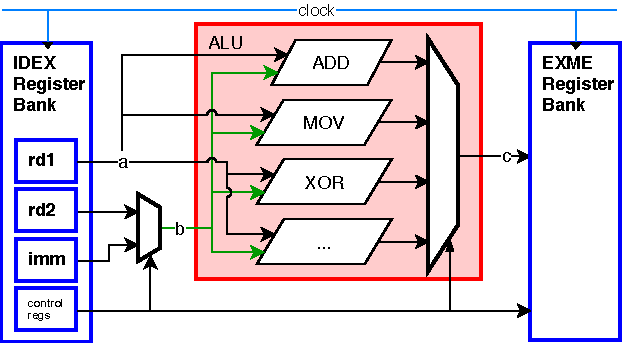
\includegraphics[width=10cm]{../img/alu}
\caption{Vmicro16 ALU diagram showing clocked inputs from the previous IDEX stage being }
\label{fig:alu}
\end{figure}

The ALU also performs comparison (\verb|CMP|) operations in which it returns flags similar to X86's overflow, signed, and zero, flags. The combination of these flags can be used to easily compute relationships between the two input operands. For example, if the zero flag is not equal to the signed flag, then the relationship between inputs $a$ and $b$ is that $a < b$.

\begin{listing}[H]
\centering
\begin{minted}[fontsize=\scriptsize,linenos,baselinestretch=0.5,frame=single,framesep=10pt]{verilog}
module branch (
    input [3:0] flags,
    input [7:0] cond,
    output reg  en
);
    always @(*)
        case (cond)
            `VMICRO16_OP_BR_U:  en = 1;
            `VMICRO16_OP_BR_E:  en = (flags[`VMICRO16_SFLAG_Z] == 1);
            `VMICRO16_OP_BR_NE: en = (flags[`VMICRO16_SFLAG_Z] == 0);
            `VMICRO16_OP_BR_G:  en = (flags[`VMICRO16_SFLAG_Z] == 0) && 
                                     (flags[`VMICRO16_SFLAG_N] == flags[`VMICRO16_SFLAG_V]);
            `VMICRO16_OP_BR_L:  en = (flags[`VMICRO16_SFLAG_Z] != flags[`VMICRO16_SFLAG_N]);
            `VMICRO16_OP_BR_GE: en = (flags[`VMICRO16_SFLAG_Z] == flags[`VMICRO16_SFLAG_N]);
            `VMICRO16_OP_BR_LE: en = (flags[`VMICRO16_SFLAG_Z] == 1) || 
                                     (flags[`VMICRO16_SFLAG_N] != flags[`VMICRO16_SFLAG_V]);
            default:            en = 0;
        endcase
endmodule
\end{minted}
\caption{ALU branch detection using flags: zero (Z), overflow (V), and negative (N).}
\end{listing}


The Verilog implementation of the ALU is shown in \cref{fig:aluv}. The ALU's asynchronous output is clocked with other registers, such as destination register \verb|rs1| and other control signals, in the \verb|EXME| register bank.
\begin{listing}[H]
\centering
\begin{minted}[fontsize=\scriptsize,linenos,baselinestretch=0.5,frame=single,framesep=10pt]{verilog}
always @(*) case (op)
    // branch/nop, output nothing
    `VMICRO16_ALU_BR,
    `VMICRO16_ALU_NOP:          c = {DATA_WIDTH{1'b0}};
    // load/store addresses (use value in rd2)
    `VMICRO16_ALU_LW,
    `VMICRO16_ALU_SW:           c = b;
    // bitwise operations
    `VMICRO16_ALU_BIT_OR:       c = a | b;
    `VMICRO16_ALU_BIT_XOR:      c = a ^ b;
    `VMICRO16_ALU_BIT_AND:      c = a & b;
    `VMICRO16_ALU_BIT_NOT:      c = ~(b);
    `VMICRO16_ALU_BIT_LSHFT:    c = a << b;
    `VMICRO16_ALU_BIT_RSHFT:    c = a >> b;
\end{minted}
\caption{Vmicro16's ALU implementation named vmicro16\_alu. vmicro16.v}
\label{fig:aluv}
\end{listing}




\subsection{Decoder Design}
Instruction decoding occurs in the between the IFID and IDEX stages. 
The decoder extracts register selects and operands from the input instruction. The decoder outputs are asynchronous which allows the register selects to be passed to the register set and register data to be read asynchronously. The register selects and register read data is then clocked into the IDEX register bank.

\begin{listing}[H]
\centering
\begin{minted}[fontsize=\scriptsize,linenos,baselinestretch=0.5,frame=single,framesep=10pt]{verilog}
always @(*) case (instr[15:11])
    `VMICRO16_OP_BR:              alu_op = `VMICRO16_ALU_BR;
    `VMICRO16_OP_MULT:            alu_op = `VMICRO16_ALU_MULT;

    `VMICRO16_OP_CMP:             alu_op = `VMICRO16_ALU_CMP;
    `VMICRO16_OP_SETC:            alu_op = `VMICRO16_ALU_SETC;
    
    `VMICRO16_OP_BIT:     casez (instr[4:0])
        `VMICRO16_OP_BIT_OR:      alu_op = `VMICRO16_ALU_BIT_OR;
        `VMICRO16_OP_BIT_XOR:     alu_op = `VMICRO16_ALU_BIT_XOR;
        `VMICRO16_OP_BIT_AND:     alu_op = `VMICRO16_ALU_BIT_AND;
        `VMICRO16_OP_BIT_NOT:     alu_op = `VMICRO16_ALU_BIT_NOT;
        `VMICRO16_OP_BIT_LSHFT:   alu_op = `VMICRO16_ALU_BIT_LSHFT;
        `VMICRO16_OP_BIT_RSHFT:   alu_op = `VMICRO16_ALU_BIT_RSHFT;
        default:                  alu_op = `VMICRO16_ALU_BAD; endcase
\end{minted}
\caption{Vmicro16's ALU implementation named vmicro16\_alu. vmicro16.v}
\caption{Vmicro16's decoder module code showing nested bit switches to determine the intended opcode. vmicro16.v}
\label{fig:vdecoder}
\end{listing}

In \cref{fig:vdecoder}, it can be seen that the first 4 opcode cases (BR, MULT, CMP, SETC) are represented using the same 15-11 (opcode) bits, however the BIT instructions share the same opcode and so require another bit range to be compared to determine the output function.



\subsection{Pipelining}
In the interim progress update, the processor design featured \textit{instruction pipelining} to meet requirement \ref{ed:ipc}. Instruction pipelining allows instructions executions to be overlapped in the pipeline, resulting in higher throughput (up to one instruction per clock) at the expense of 5-6 clocks of latency and \textit{significant} code complexity. As the development of the project shifted from single-core to multi-core, it became obvious that the complexity of the pipelined processor would inhibit the integration of multi-core functionality. It was decided to remove the instruction pipelining functionality and use a simpler state-machine based pipeline that is much simpler to extend and would cause fewer challenges later in the project. 

\subsection{Design Optimisations}
In a design that has many instantiations of the same component, a small resource saving improvement within the component can have a significant overall savings improvement if it is instantiated many times. Project requirement \ref{cd:vendor} requires the design to be compiled for a range of FPGA sizes, and so space saving optimisations are considered. 

\subsubsection{Register Set Size Improvements}
A register set in a CPU is a fast, temporary, and small memory that software instructions directly manipulate to perform computation. In the Vmicro16 instruction set, eight registers named r0 to r7 are available to software. The instruction set allows up to two registers to be references in most instructions, for example the instruction \verb|add r0, r1| tells the processor to perform the following actions:
\begin{enumerate}[leftmargin=4\parindent, label=\bfseries Clock \arabic*.]
\item Fetch r0 and r1 from the register set
\item Add the two values together in the ALU
\item Store the result back the register set in r0
\end{enumerate}
For Clock 1, it was originally decided to use a dual port register set (meaning that two data reads can be performed in a single clock, in this case r0 and r1), however due to the asynchronous design of the register set (for speed) the RTL produced consumed a significant amount of FPGA resources, approximately 256 flip-flops (16 (data width) * 8 (registers) * 2 (ports)). To reduce this, it was decided to split task 1 into two steps over two clock cycles using a single-port register set. This required the processor pipe-line to use another clock cycle resulting in slightly lower performance, however the size improvements will allow for more cores to be instantiated in the design. This optimisation is also applied to the interrupt register set, resulting in a saving of approximately 256 flip-flops per core (128 in the normal mode register set, and 128 in the interrupt register set). As shown, adding a single clock delay saves a significant amount of LUTs. This saving will be amplified in designs with many cores.



\section{Interrupts}
\label{sect:interrupts}
Interrupts are a technique used by processors to run software functions when an event occurs within the processor, such as exceptions, or signalled from an external source, such as a UART receiver signalling it has received new data. Today, it is common for micro-controllers, soft-processors, and desktop processors, to all feature interrupts. Modern implementations support an \textit{interrupt vector} which is a memory array that contains addresses to different \textit{interrupt handlers} (a software function called when a particular interrupt is received).

Although interrupts are not a requirement for a multi-core system, it was decided to implement this functionality to boost my understanding of such systems. In addition, example demos provided with this project are better visualised with a interrupt functionality.

\subsection{Overview}
The interrupt functionality in this project supports the following:
\begin{itemize}
\item Per-core 8 cell interrupt vector accessible to software.\\
Software programs running on the Vmicro16 processor can edit the interrupt vector to add their own interrupt handlers at runtime.

\item Fast context switching.\\
A dedicated interrupt register set is multiplexed with the normal mode register set to provide faster context switching. It should be noted that only the registers are saved during a context switch. The means that the stack is not saved. A schematic of the register multiplex is shown in \cref{fig:regmult}.

\item Parametrised interrupt sources and widths.\\
Users can configure the width of the interrupt in signals and the data width per interrupt source via the \verb|vmicro16_soc_config.v|. By default, 8 interrupt sources are available and each can provide 8-bits of data.
\end{itemize}

\subsection{Hardware Implementation}

\subsubsection{Context Switching}
When acting upon an incoming interrupt the current state the processor must be saved so that changes from the interrupt handler, such as register writes and branches, do not affect the current state. After the interrupt handler function signals it has finished (by using the \textit{Interrupt Return} \verb|INTR| instruction) the saved state is restored.
In the case of the Vmicro16 processor, the program counter \verb|r_pc[15:0]| and register set \verb|regs| instance are the only states that are saved. Going forth, the terms \textit{normal mode} and \textit{interrupt mode} are used to describe what registers the processor should use when executing instructions.

When saving the state, to avoid clocking 128 bits (8 registers of 16 bits) into another register (which would increase timing delays and logic elements), a dedicated register set for the interrupt mode (\verb|regs_isr|) is multiplexed with the normal mode register set (\verb|regs|). Then depending on the mode (identified by the register \verb|regs_use_int|) the processor can easily switch between the two large states without significantly affecting timing.

The timing diagram in \cref{fig:interrupts} shows the behavioural logic for the TIMR0 interrupt source.

\begin{figure}[H]
\centering
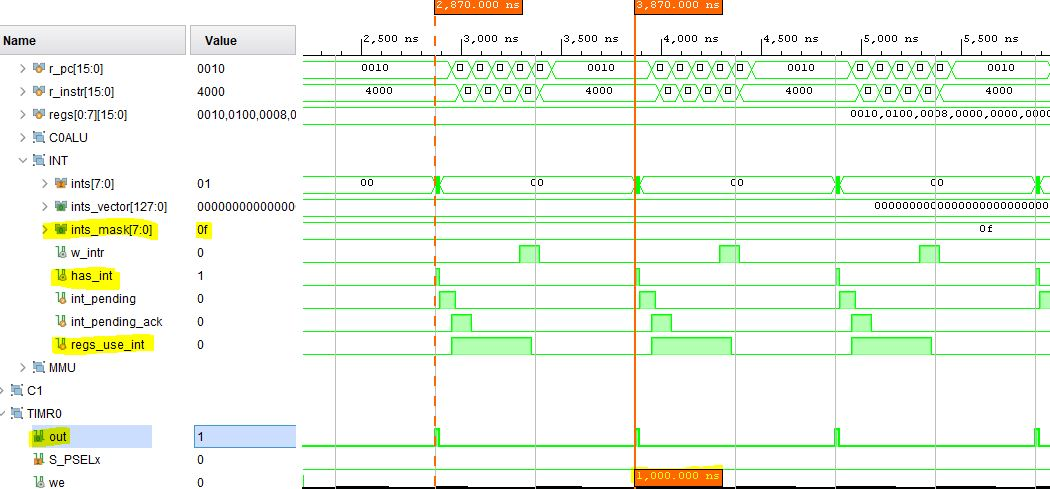
\includegraphics[width=\textwidth]{interrupts}
\caption{Time diagram showing the TIMR0 peripheral emitting a 1us periodic interrupt signal (out) to the processor. The processor acknowledges the interrupt (int\_pending\_ack) and enters the interrupt mode (regs\_use\_int) for a period of time. When the interrupt handler reaches the Interrupt Return instruction (indicated by w\_intr) the processor returns to normal mode and restores the normal state.}
\label{fig:interrupts}
\end{figure}

\subsection{Software Interface}
A memory-mapped software interface is provided through the MMU to allow easy software control of the interrupt behaviour. The interface is provided at the address range 0x0100 to 0x0108. This interface is per-core allowing each core to individually control what interrupts it receives and what functions to call upon an interrupt. This enables complex functionality, such as allowing each core to execute different functions upon the same interrupt.

\begin{figure}[H]
\centering
\begin{bytefield}[bitwidth=4ex, rightcurly=., rightcurlyspace=0pt]{16}
\bitheader[endianness=big]{0-15} \\
\begin{rightwordgroup}{0100 RW}
\bitbox{16}{Interrupt handler $0$}
\end{rightwordgroup} \\

\bitbox[]{16}{$\vdots$ \\[1ex]} \\
\begin{rightwordgroup}{0107 RW}
\bitbox{16}{Interrupt handler $7$}
\end{rightwordgroup} \\

\begin{rightwordgroup}{0108 RW}
\bitbox{8}{\color{lightgray}\rule{\width}{\height}} & \bitbox{8}{Interrupt bit mask}
\end{rightwordgroup}
\end{bytefield}
\caption{The interrupt vector (0x0100 - 0x0107) consists of eight 16-bit values that point to memory addresses of the instruction memory to jump to.}
\label{fig:r_interrupts}
\end{figure}

\subsubsection{Interrupt Vector (0x0100-0x0107)}
The interrupt vector is a per-core register that is used to store the addresses of interrupt handlers. An interrupt handler is simply a software function residing in instruction memory that is branched to when a particular interrupt is received. 

\subsubsection{Interrupt Mask (0x0108)}
The interrupt mask is a per-core register that is used to mask/listen specific interrupt sources. This enables processing cores to individually select which interrupts they respond to. This allows for multi-processor designs where each core can be used for a particular interrupt source, improving the time response to the interrupt for time critical programs. The Interrupt Mask register is an 8-bit read/write register where each bit corresponds to a particular interrupt source and each bit corresponds with the interrupt handler in the interrupt vector. The interrupt mask register is shown in \cref{fig:r_interruptmask}.

\begin{figure}
\centering
\begin{bytefield}[bitwidth=4ex]{16}
& \bitlabel{8}{} &
& \bitlabel{6}{[7:2] User defined} &
& \bitlabel{1}{UART0 RX} 
& \bitlabel{1}{TIMR0} \\
\bitheader[endianness=big]{0-7,8,15} \\
  \bitbox{8}{\color{lightgray}\rule{\width}{\height}}
& \bitbox{1}{0}
& \bitbox{1}{0}
& \bitbox{1}{0}
& \bitbox{1}{0}
& \bitbox{1}{0}
& \bitbox{1}{0}
& \bitbox{1}{0}
& \bitbox{1}{0}
\end{bytefield}
\caption{Interrupt Mask register (0x0108). Each bit corresponds to an interrupt source. 1 signifies the interrupt is enabled for/visible to the core. Bits [7:2] are left to the designer to assign. Bit 0 is assigned to TIMR0's interval timer. Bit 1 is assigned to the UART0's receiver (unassigned if DEF\_USE\_REPROG is enabled).}
\label{fig:r_interruptmask}
\end{figure}

\subsubsection{Software Example}
To better understand the usage of the described interrupt registers, a simple software program is described below. The following software program produces a simple and power efficient routine to initialise the interrupt vector and interrupt mask.

% pip install pygments-arm
\begin{minted}[fontsize=\footnotesize,linenos,,baselinestretch=0.8]{arm}
setup_interrupts:
    // Set interrupt vector at 0x100
    // Move address of isr0 function to vector[0]
    movi    r0, isr0
    // create 0x100 value by left shifting 1 8 bits
    movi    r1, #0x1
    movi    r2, #0x8
    lshft   r1, r2
    // write isr0 address to vector[0]
    sw      r0, r1
    
enable_interrupts:
    // enable all interrupts by writing 0x0f to 0x108
    movi    r0, #0x0f
    sw      r0, r1 + #0x8 // (0x100 + 0x8 = 0x108)
    halt                  // enter low power idle state
    
isr0:                     // arbitrary name
    movi    r0, #0xff     // do something
    intr                  // return from interrupt
\end{minted}

A more complex example software program utilising interrupts and the TIMR0 interrupt is described in section \ref{sec:2coretimer}.

\subsection{Design Improvements}
The hardware and software interrupt design have changed throughout the projects cycle. In initial versions of the interrupt implementation, the software program, while waiting for an interrupt, would be in a tight infinite loop (branching to the same instruction). This resulted in the processor using all pipeline stages during this time. The pipeline stages produce many logic transitions and memory fetches which raise power consumption and temperatures. This is quite noticeable especially when running on the Spartan-6 LX9 FPGA.

To improve this, it was decided to implement a new state within the processor's state machine that, when entered, did not produce high frequency logic transitions or memory fetches. The \verb|HALT| instruction was modified to enter this state and the only way to leave is from an interrupt or top-level reset. This removes the need for a software infinite loop that produces high frequency logic transitions (decoding, ALU, register reads, etc.) and memory fetches.





\section{Verification}
Various verification techniques are employed to ensure correct operation of the processor.

The first technique involves using static assertions to identify incorrect configuration parameters at compile time, such as having zero instruction memory and scratch memory depth. These assertions use the \verb|static_assert| for top level checks and \verb|static_assert_ng| for checks inside \verb|generate| blocks.

The second verification technique is to use assertions in \verb|always| blocks to identify incorrect behavioural states. This is done using the \verb|rassert| (run-time assert) macro.

The third verification technique is to use automatic verifying test benches. These test benches drive components of the processor, such as the ALU and decoder, and check the output against the correct value. This uses the \verb|rassert| macro.

The final method of verification is to verify the complete design via a behavioural test bench. The design is passed a compiled software program with a known expected output, and is ran until the \verb|r_halt| signal is raised. The test bench then checks the value on the \verb|debug0|, \verb|debug1|, and \verb|debug2| signals against the expected value. If this matches, then it is assumed that sub-components of the design also operate correctly. This technique does not monitor the states of sub-components and statistics (such as time taken to execute an instruction), there leaves the possibility that some components could have entered an illegal state.





